\section{Zusammenfassung der Daten}

Zur Evaluation des Prototypen wurde mit drei Probanden das Thinking Aloud Verfahren in Kombination mit dem TLX-Test verwendet. Die Daten der TLX-Tests der einzelnen Probanden sind in den Tabellen \ref{tab:tlx-proband1}, \ref{tab:tlx-proband2} und \ref{tab:tlx-proband3} aufgelistet.

% TLX-Daten Proband 1
\begin{table}[htb]
    \caption{\label{tab:tlx-proband1}Daten des TLX-Tests für Proband 1.}
    \centering
    \begin{tabular}{l r r}
        Proband 1 & Bewertung & Wichtung \\
        \hline
        Geistige Anforderung & 20 & 0.06666667 \\
        Körperliche Anforderung & 5 & 0 \\
        Zeitliche Anforderung & 85 & 0.2 \\
        Leistung & 40 & 0.26666667 \\
        Anstrengung & 20 & 0.13333333 \\
        Frustration & 85 & 0.33333333 \\
        \hline
        Gesamtbeanspruchung & 60.00 & \\
    \end{tabular}
\end{table}

% TLX-Daten Proband 2
\begin{table}[htb]
    \caption{\label{tab:tlx-proband2}Daten des TLX-Tests für Proband 2.}
    \centering
    \begin{tabular}{l r r}
        Proband 1 & Bewertung & Wichtung \\
        \hline
        Geistige Anforderung & 35 & 0.2 \\
        Körperliche Anforderung & 10 & 0.13333333 \\
        Zeitliche Anforderung & 30 & 0.06666667 \\
        Leistung & 65 & 0.13333333 \\
        Anstrengung & 20 & 0.2 \\
        Frustration & 55 & 0.26666666 \\
        \hline
        Gesamtbeanspruchung & 37.67 & \\
    \end{tabular}
\end{table}

% TLX-Daten Proband 3
\begin{table}[htb]
    \caption{\label{tab:tlx-proband3}Daten des TLX-Tests für Proband 3.}
    \centering
    \begin{tabular}{l r r}
        Proband 1 & Bewertung & Wichtung \\
        \hline
        Geistige Anforderung & 25 & 0.06666667 \\
        Körperliche Anforderung & 5 & 0.2 \\
        Zeitliche Anforderung & 25 & 0.2 \\
        Leistung & 30 & 0.06666667 \\
        Anstrengung & 35 & 0.13333333 \\
        Frustration & 35 & 0.33333333 \\
        \hline
        Gesamtbeanspruchung & 26.00 & \\
    \end{tabular}
\end{table}

Die absoluten (Abbildung \ref{fig:absolut}) und relativen, auf 1 normierten, (Abbildung \ref{fig:relativ}) Werte aus den TLX-Tests der Probanden wurden gegenübergestellt.

% Absolute Beanspruchungen
\begin{figure}[htb]
    \centering
    \subfigure[\label{fig:absolut}Gegenüberstellung der absoluten Beanspruchungen der Probanden aus den TLX-Tests.]{
        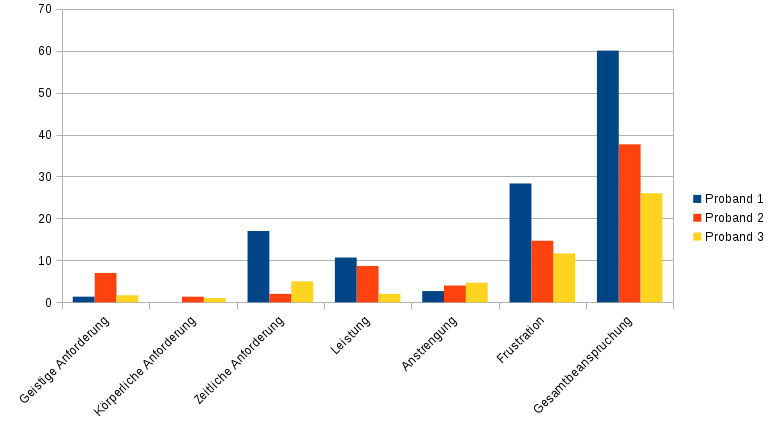
\includegraphics[width=\textwidth]{../diagramme/absolute_beanspruchung.png}
    }

    \subfigure[\label{fig:relativ}Gegenüberstellung der relativen Beanspruchungen der Probanden aus den TLX-Tests durch Normierung der Gesamtbeanspruchung auf 1.]{
        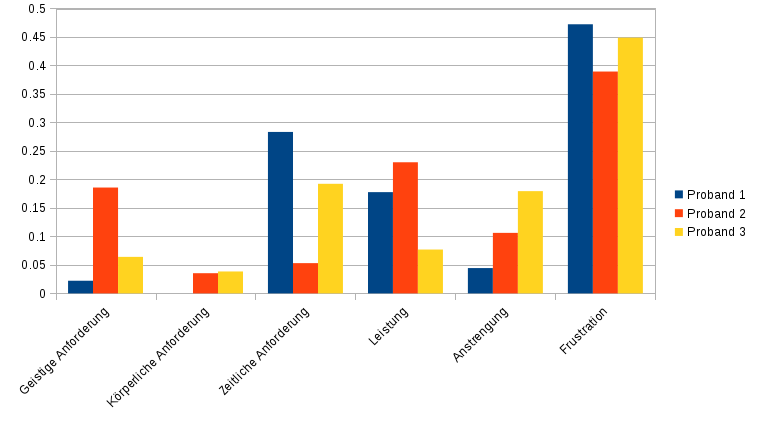
\includegraphics[width=\textwidth]{../diagramme/relative_beanspruchung.png}
    }
\end{figure}
